\section{模型四：二类潜在语音表型辅助分型}

\subsection{建模边界}

题目第四问涉及运动型和非运动型帕金森病，但给定数据没有真实运动型/非运动型临床标签。因此，本文不训练真实临床亚型监督分类器，而是在 Dataset 1 的 188 名 PD 受试者内部进行 \(k=2\) 无监督聚类，得到基于语音特征的二类潜在表型。该结果可作为探索性辅助分型线索，不能等同于真实临床亚型诊断。

\subsection{输入、方法与结果}

候选输入特征集包括 Top20、Top50、all acoustic 以及 PD-only 内部筛选得到的相关性去冗余、高 IQR/MAD 和 SparsePCA 表示方案。综合内部聚类指标、簇均衡性和 10000 组 Dirichlet 权重敏感性分析后，本文采用多候选报告口径。\feature{top20_biomarkers} / \feature{pca_5} / KMeans 的 top-1 频率最高，为 37.3\%，低于 60\% 的稳健主推荐阈值，因此表述为“相对推荐候选方案”，不作为唯一最优结论。

所有候选方案先执行标准化，再按方案进行 PCA 和聚类。聚类输入不包含 \feature{id}、\feature{gender}、\feature{class}、\feature{sex_male}、\feature{record_count} 或任何标签列。聚类质量通过 silhouette、Calinski-Harabasz、Davies-Bouldin 和重采样 ARI 等指标综合评价\upcite{silhouette,calinski,davies,ari}。

\begin{table}[H]
\centering
\caption{二类潜在语音表型相对推荐候选方案}
\begin{tabularx}{\textwidth}{lYccc}
\toprule
候选方案 & 特征 / 表示 / 聚类方法 & top-1 频率 & top-3 频率 & 判定 \\
\midrule
候选 1 & \feature{top20_biomarkers} / \feature{pca_5} / KMeans & 37.3\% & 63.2\% & 相对推荐 \\
候选 2 & \feature{top50_biomarkers} / \feature{pca_5} / KMeans & 22.4\% & 35.2\% & 可接受候选 \\
候选 3 & \feature{pd_high_iqr_top50} / \feature{pca_5} / AgglomerativeClustering & 21.0\% & 28.9\% & 可接受候选 \\
\bottomrule
\end{tabularx}
\end{table}

\begin{table}[H]
\centering
\caption{二类潜在语音表型相对推荐方案指标}
\begin{tabularx}{\textwidth}{lY}
\toprule
项目 & 数值 \\
\midrule
相对推荐候选方案 & \feature{top20_biomarkers} / \feature{pca_5} / KMeans \\
PD 受试者数 & 188 \\
Cluster 0 人数 & 62 \\
Cluster 1 人数 & 126 \\
Smaller cluster ratio & 0.3298 \\
Silhouette & 0.3674 \\
Stability ARI mean & 0.9897 \\
权重敏感性 top-1 频率 & 37.3\% \\
\bottomrule
\end{tabularx}
\end{table}

\begin{figure}[H]
\centering
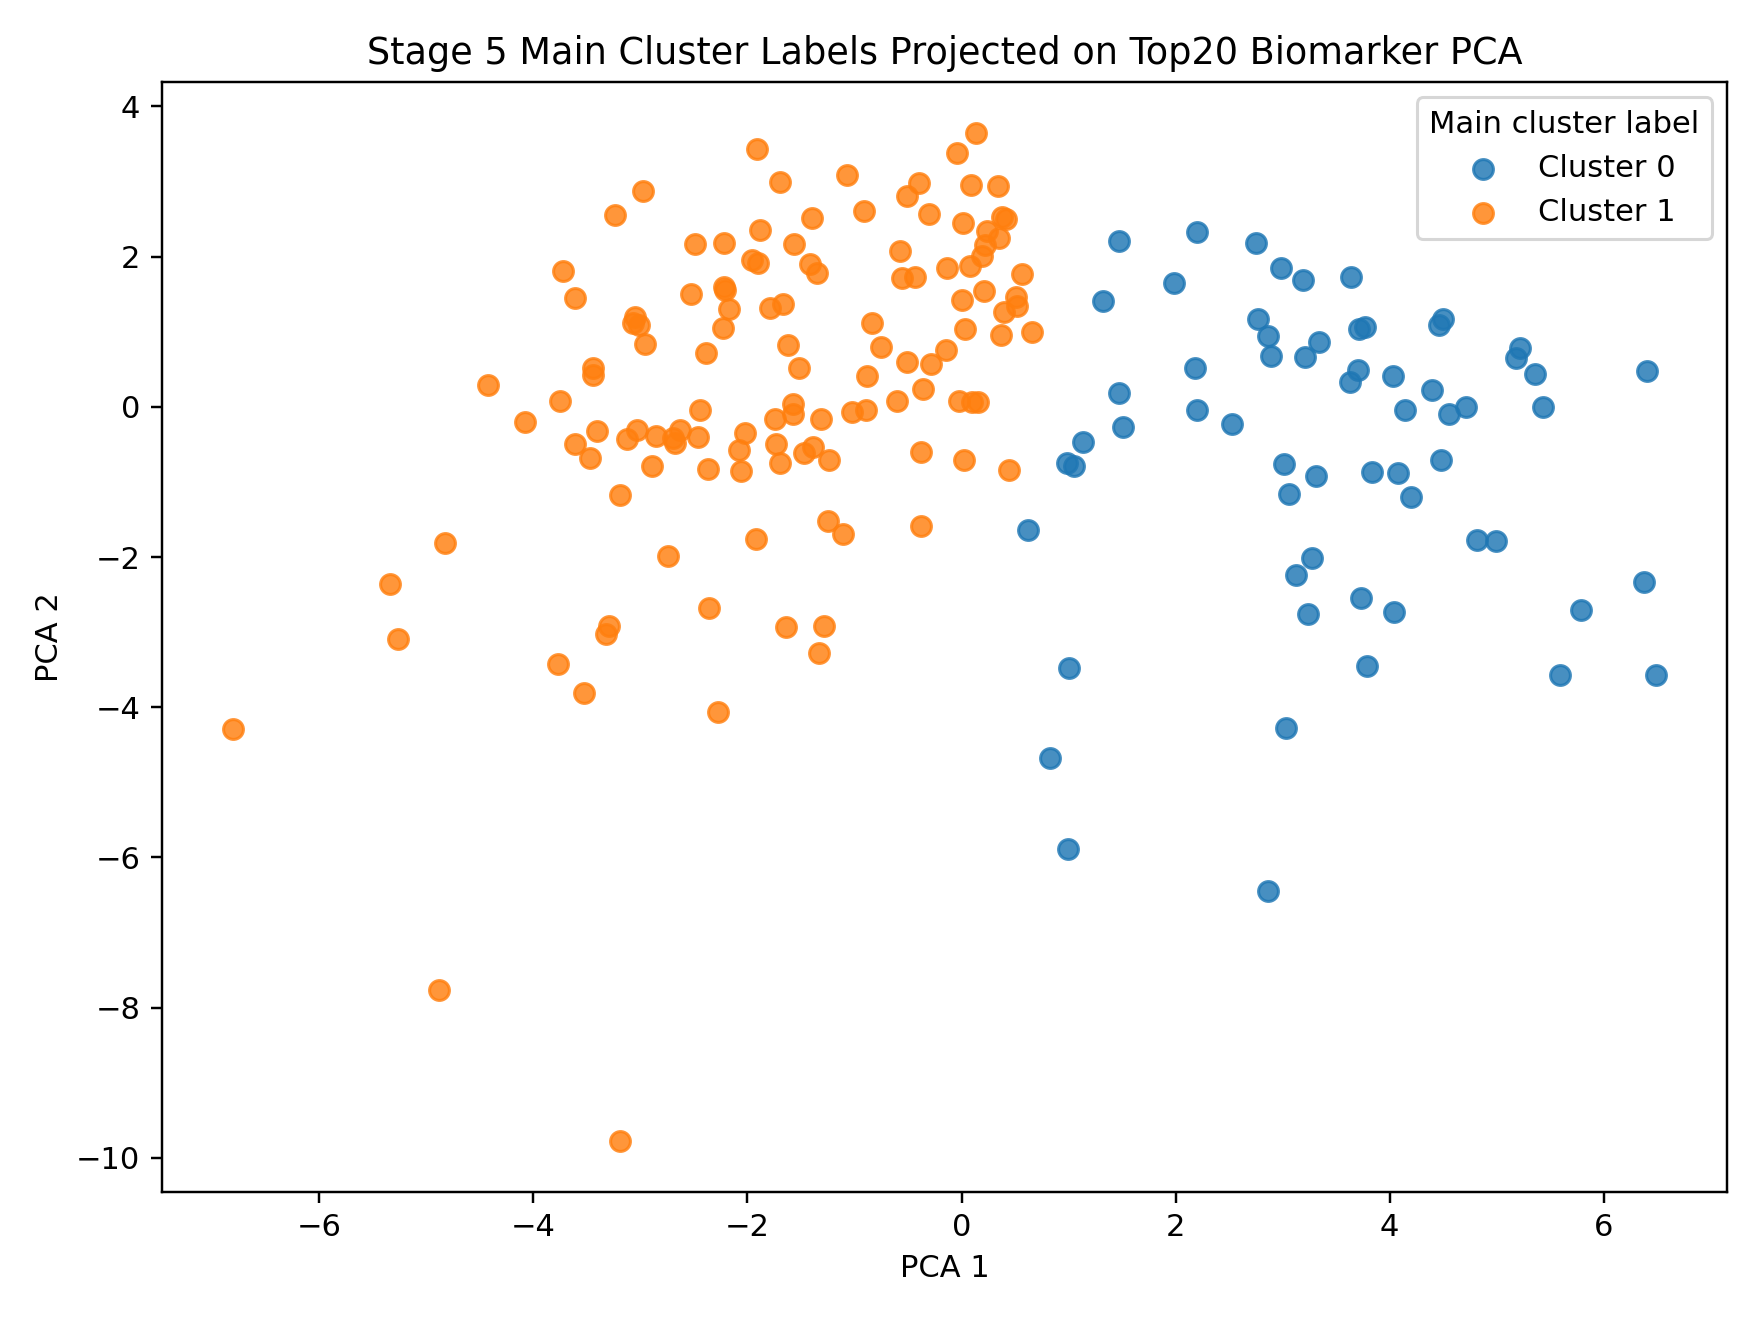
\includegraphics[width=0.82\textwidth]{figures/stage5_pca_k2_clusters_top20.png}
\caption{Dataset 1 PD 受试者二类潜在语音表型 PCA 可视化}
\end{figure}

该图将相对推荐候选方案得到的二类聚类标签投影到 Top20 特征的前两个 PCA 方向上。图中两类样本在二维空间中呈现较明显的左右分离趋势，说明 Top20 候选特征能够支持 PD 受试者内部的二类潜在语音表型划分。但 PCA 二维图只是可视化投影，不能替代 silhouette、簇规模和稳定性 ARI 等定量指标，也不能直接说明真实临床亚型存在。

\begin{figure}[H]
\centering
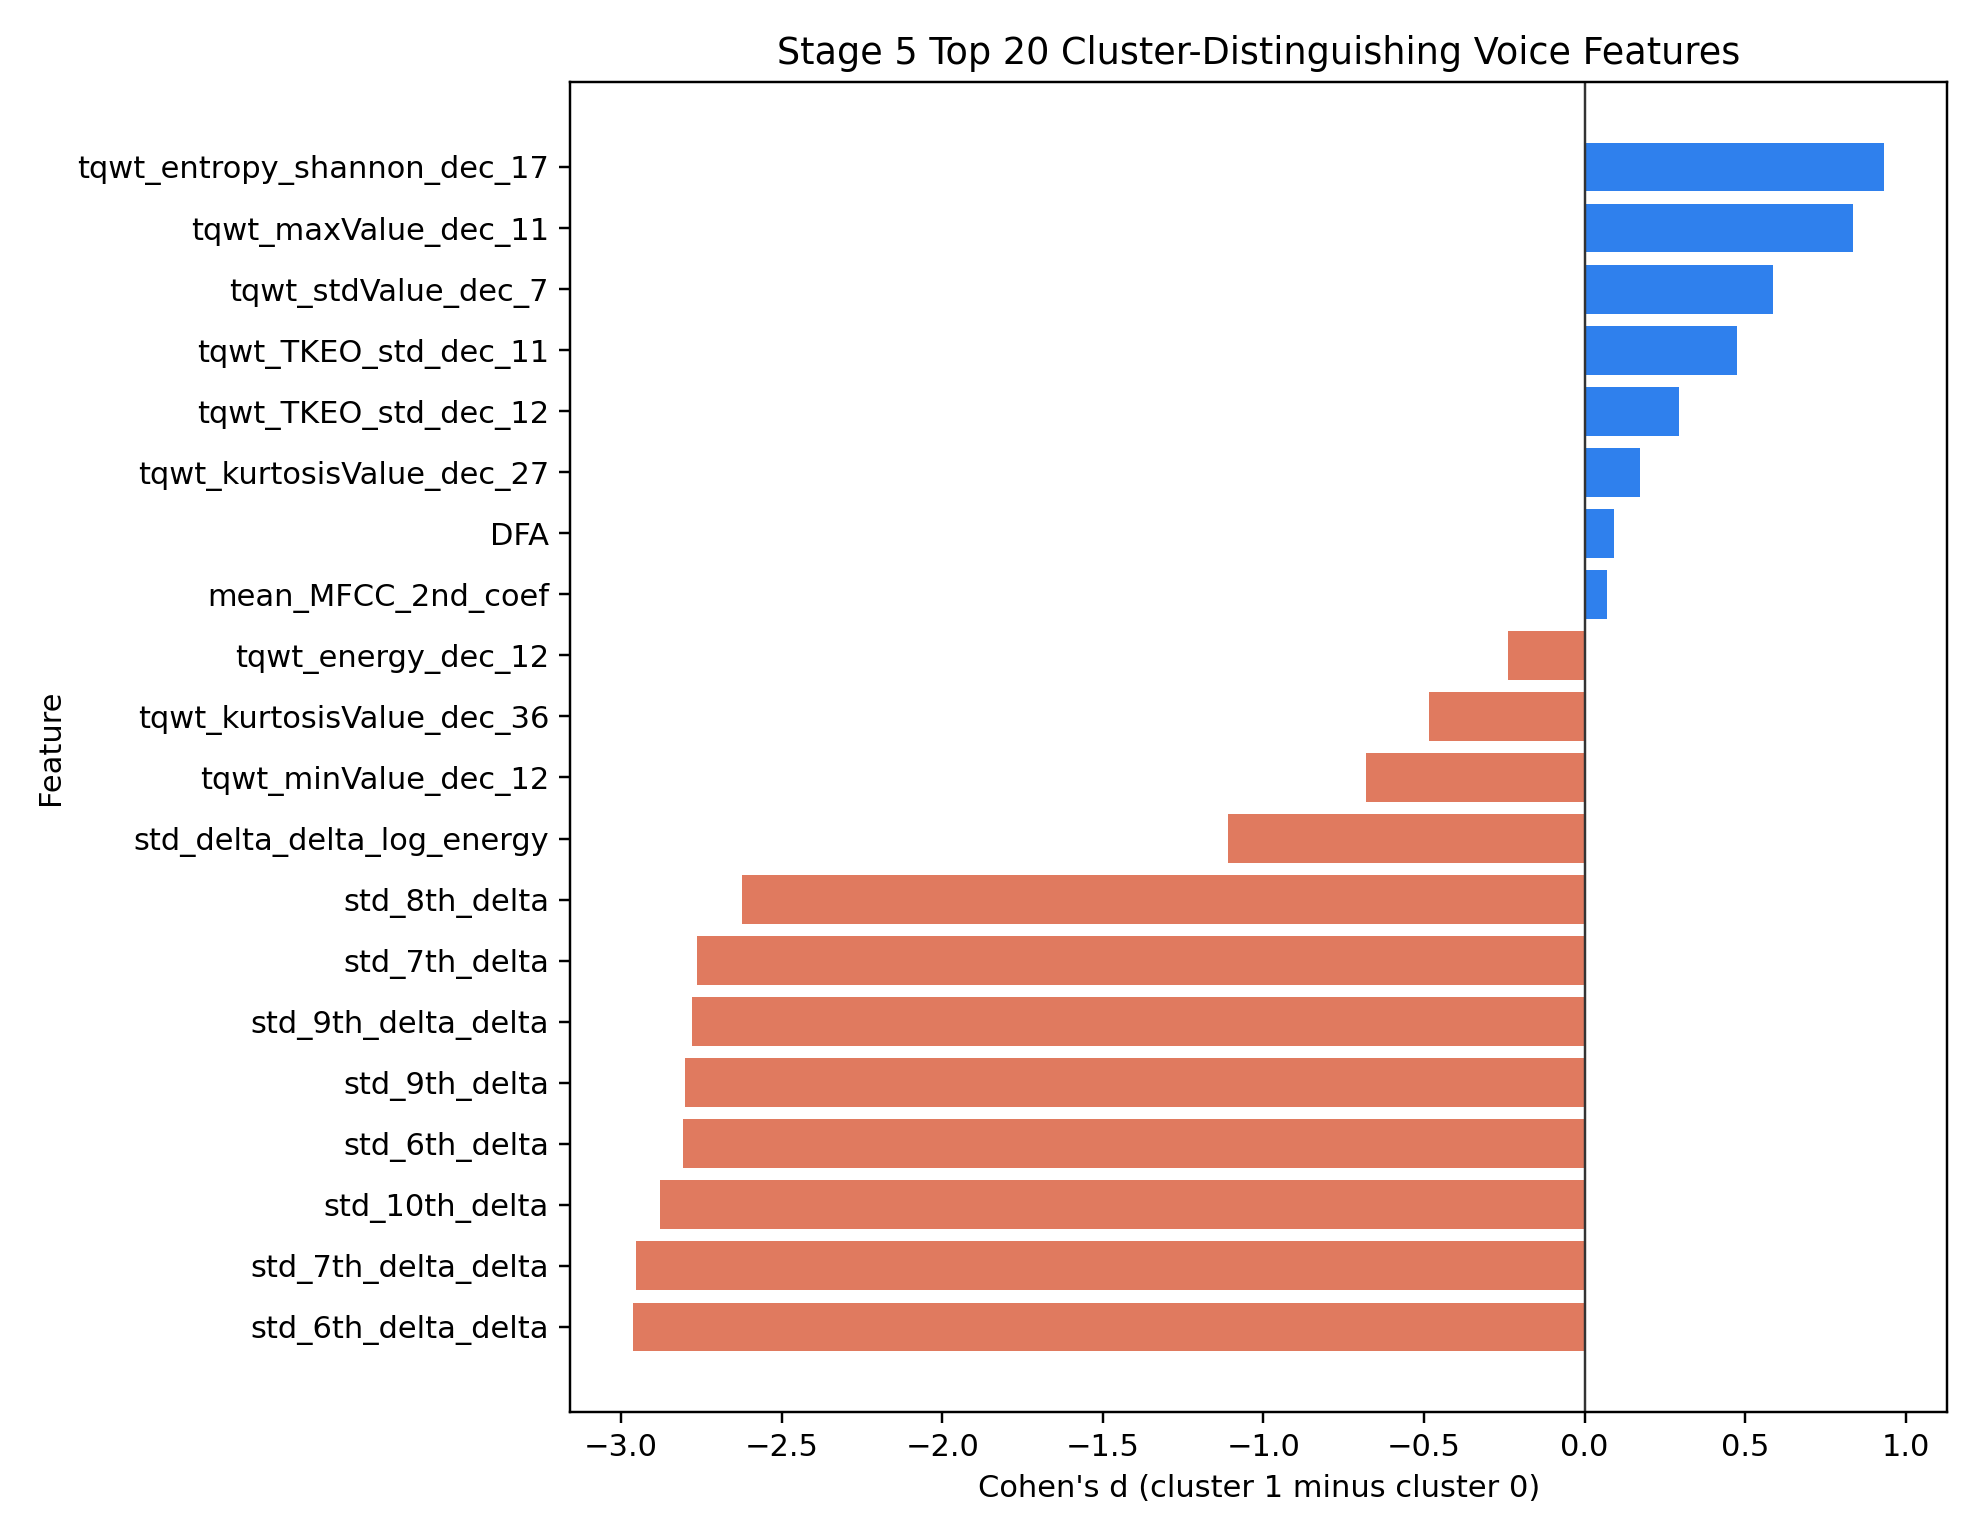
\includegraphics[width=0.88\textwidth]{figures/stage5_cluster_feature_difference_top20.png}
\caption{二类潜在语音表型的 Top20 特征差异}
\end{figure}

该图以 Cohen's \(d\) 展示二类潜在表型在 Top20 特征上的差异方向。横轴为 cluster 1 minus cluster 0，因此负值表示 cluster 0 更高，正值表示 cluster 1 更高。图中 cluster 0 在多项 Delta / Delta-delta 动态谱波动特征上更高，cluster 1 在若干 TQWT 特征上更高，提示两簇主要反映动态谱波动和多尺度声学结构的差异。该差异只能解释为语音表型差异，不能直接解释为真实运动型/非运动型临床差异。

\subsection{表型解释}

相对推荐候选方案得到 cluster 0 共 62 人、cluster 1 共 126 人。cluster 0 在多项 Delta / Delta-delta 动态谱波动特征上更高，例如 \feature{std_6th_delta_delta}、\feature{std_7th_delta_delta}、\feature{std_10th_delta}、\feature{std_6th_delta} 等。cluster 1 在部分 TQWT 多尺度特征上更高，例如 \feature{tqwt_entropy_shannon_dec_17}、\feature{tqwt_maxValue_dec_11}、\feature{tqwt_stdValue_dec_7}、\feature{tqwt_TKEO_std_dec_11} 等。

后续聚类标签复现模型学习的是上述无监督聚类标签，用于将探索性分型规则模型化。该分类器不是根据真实运动型/非运动型标签训练，不能解释为真实临床亚型诊断性能。
